\section{Relations Between Conjectures}

\begin{frame}[label=relations]{Relations}
\begin{mypic}
\begin{scope}[scale=0.75,transform shape]
\tikzstyle{r}=[rectangle,inner sep=1mm,draw,text centered, text width=44mm,minimum height=20mm]

\node[r,text width=28mm] (w) at (5.5,4) {\small Weak Greedy\\ Hierarchical Conjecture\\};
\node[r] (cc) at (0,7) {\small Collapsing\\ Conjecture\\}; 
\node[r] (gc) at (0,1) {\small Greedy\\ Conjecture\\};
\node[r] (ghc) at (0,4) {\small Greedy Hierarchical\\ Conjecture\\}; 

\node[r, text width=39mm] (ca) at (10,7) {\small Collapsing Algo is 2-approx\\};
\node[r, text width=39mm] (gha) at (10,4) {\small Greedy Hierarchical Algo is 2-approx\\};
\node[r, text width=39mm] (ga) at (10,1) {\small Greey Algo is 2-approx\\};

%\draw[help lines] (0,0) grid (14,6);

\foreach \f/\t in {cc.east/w, ghc/w, gc.east/w}
  \draw[->] (\f) -- (\t);
  
\draw[<->] (cc) -- (ghc);
  
\foreach \f/\t in {cc/ca, w/gha, gc/ga}
  \draw[dashed,->] (\f) -- (\t);
 
\end{scope}
%\foreach \f/\t in {cc/ca, cc/w, gc/ga, gc/w, w/gha, ga/gha}
 % \draw[->] (\f) -- (\t);
\end{mypic}
\end{frame}

\begin{frame}{Supporting Conjectures}
\begin{itemize}
\item All the conjectures hold for the special case when input strings have length at most three
\item The conjectures have been verified on millions of datasets (both handcrafted and randomly generated)
\end{itemize}
\end{frame}

\begin{frame}{Framework}
A framework for visualizing and verifying the conjectures:
\alert{\url{compsciclub.ru/scs}}

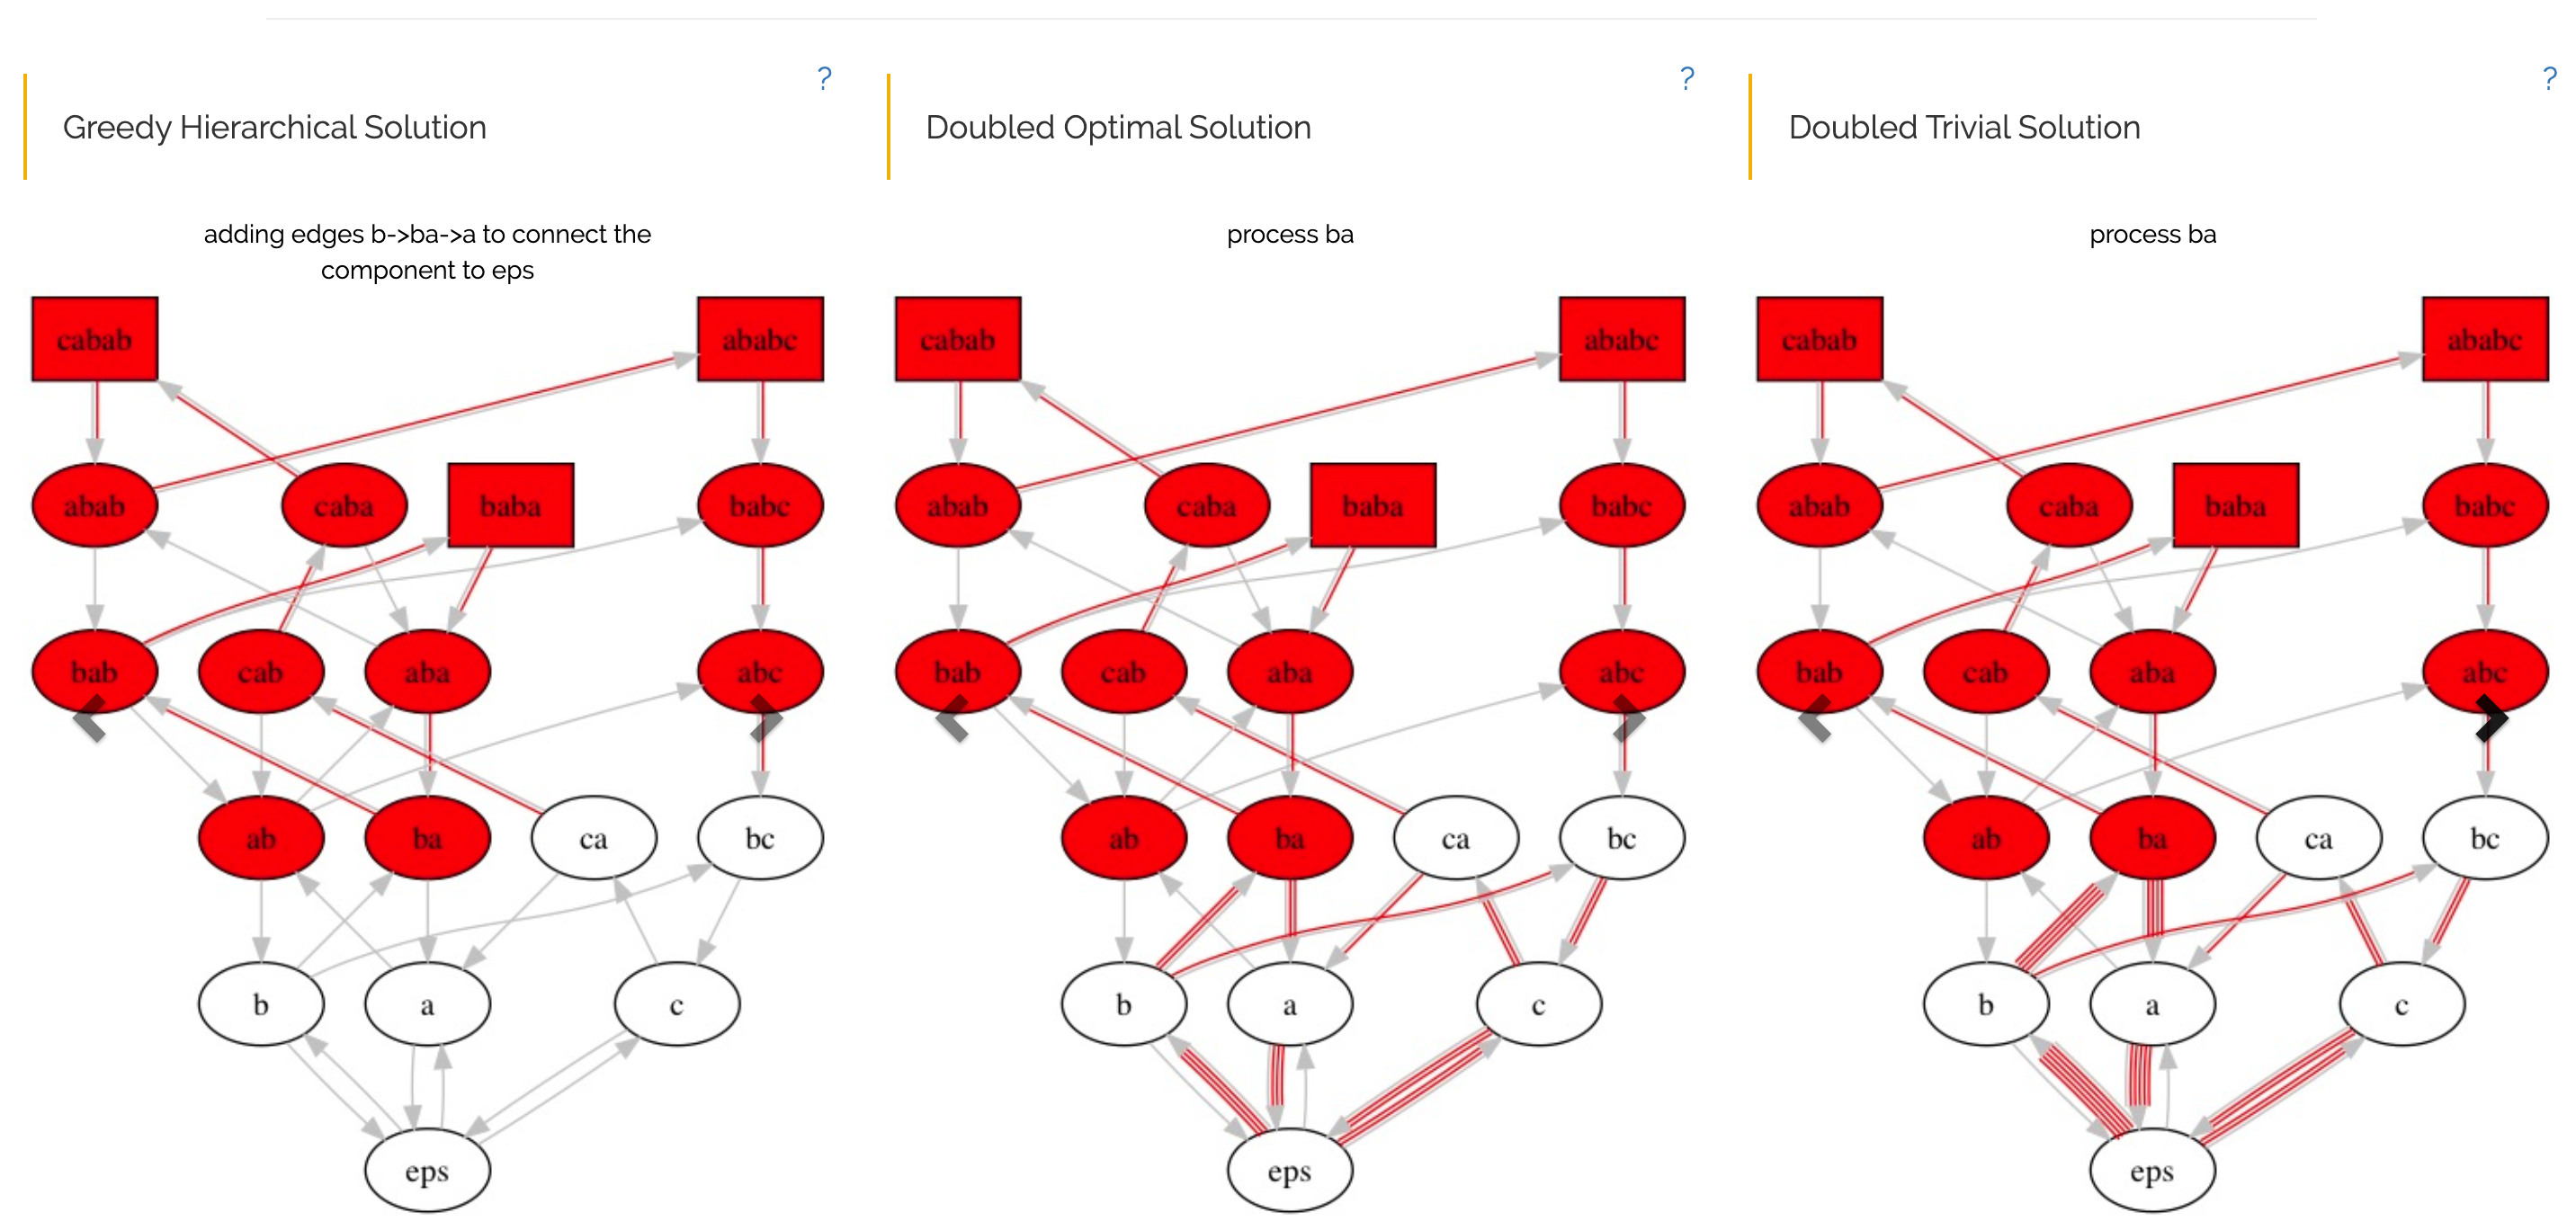
\includegraphics[width=\textwidth]{framework.png}
\end{frame}